\documentclass[table,x11names,aspectratio=169]{beamer}
% \documentclass[handout,table]{beamer}

\usepackage[utf8]{inputenc}
\usepackage[spanish]{babel}
\usepackage{pbox}
\usepackage{tikz}
\usepackage{mathabx}
\usepackage{beamerthemeshadow}
\usepackage{times}
\usepackage{enumerate}
\usepackage{graphicx}
\usepackage{graphics}
\usepackage{listings}
\usepackage{multicol}
\usepackage{amsmath,amssymb,amsfonts,latexsym,stmaryrd}
\usepackage{tabularx}
\usepackage{colortbl}
\usepackage{xcolor,pgf}% http://ctan.org/pkg/{listings,xcolor,transparent}
\usepackage{ragged2e} % para justificar texto
\usepackage{textcomp} % Para usar simbolos en texto tipo +- etc
\usepackage{siunitx}
\usepackage{../res/lstlangarm}
\usepackage[absolute,overlay]{textpos}
  \setlength{\TPHorizModule}{1mm}
  \setlength{\TPVertModule}{1mm}
\usepackage{shadow}


\usetikzlibrary{calc}
\pgfdeclarelayer{background}
\pgfdeclarelayer{foreground}
\pgfsetlayers{background,main,foreground}


\mode<presentation>{
% 	\usetheme{Warsaw}
% 	\usetheme{Ilmenau}
	\usetheme{Copenhagen}
	\useoutertheme{infolines}
}

\setbeamercovered{invisible}
\setbeamertemplate{navigation symbols}{}


\author{Alejandro Furfaro}
% \title{Organización del Computador II}
% \title{Técnicas Digitales III}
\title{ARMv7 - Gestión de Interrupciones}
% \institute{Departamento de Computación - FCEyN - UBA}
% \institute{Departamento de Electrónica - UTN.BA}
\date{\today}

\graphicspath
{
  {../img/}
}

\newcounter{saveenumi}
\newcommand{\seti}{\setcounter{saveenumi}{\value{enumi}}}
\newcommand{\conti}{\setcounter{enumi}{\value{saveenumi}}}
\resetcounteronoverlays{saveenumi}

\begin{document}

\lstset{
	frame=Ltb,
	framerule=0pt,
	aboveskip=0.5cm,
	framextopmargin=3pt,
	framexbottommargin=3pt,
	framexleftmargin=0.4cm,
	framesep=0pt,
	rulesep=.4pt,
	backgroundcolor=\color{gray97},
	rulesepcolor=\color{black},
	language=[ARM]Assembler,
	captionpos=b,
	tabsize=6,
	frame=lines,
	keywordstyle=\color{blue},
	commentstyle=\color{purple},
	stringstyle=\color{red},
	numbers=left,
	numberstyle=\tiny,
	numbersep=5pt,
	breaklines=true,
	showstringspaces=false,
	basicstyle=\footnotesize,
	emph={label},
}

\begin{figure}[ht!]
  \centering
  
\includegraphics [width =0.4 \textwidth ]{ARM-Cortex.jpg}
\end{figure}
\vspace{-2cm}
\titlepage

\definecolor{OliveGreen}{RGB}{2,80,1}
\definecolor{LigthOrange}{RGB}{255,255,200}
\definecolor{gray97}{gray}{.97}
\definecolor{Gray}{RGB}{171,174,178}
\definecolor{orange}{RGB}{255,127,0}

\AtBeginSubsection[]
{
\begin{frame}[t]{Contenido}
    \setcounter{tocdepth}{2}  
    \footnotesize
    \tableofcontents[currentsection, currentsubsection, sectionstyle=show/shaded, subsectionstyle=show/shaded]
\end{frame}
}
  
\begin{frame}[t]{Contenido}
    \setcounter{tocdepth}{2} 
    \footnotesize
    \tableofcontents
\end{frame}

%%%%%%%%%%%%%%%%%%%%%%%%%%%%%%%%%%%%%%%%%%%%%%%%
%Template de aqui en mas ;)
%%%%%%%%%%%%%%%%%%%%%%%%%%%%%%%%%%%%%%%%%%%%%%%%
\pgfdeclareimage[height=0.9cm]{left-logo}{}
\pgfdeclareimage[height=0.5cm]{right-logo}{ARM-Cortex.jpg}
\logo{\pgfuseimage{right-logo}}
\setbeamertemplate{sidebar left}
{
\logo{\pgfuseimage{left-logo}}
\vfill%
\rlap{\hskip0.1cm\insertlogo}%
\vskip15pt%
}
%%%%%%%%%%%%%%%%%%%%%%%%%%%%%%%%%%%%%%%%%%%%%%%%
\definecolor{OliveGreen}{RGB}{2,80,1}
\definecolor{Gray}{RGB}{171,174,178}
\definecolor{gray97}{gray}{.97}

\section{Introducción}
\subsection{Interrupciones en Microprocesadores}
\begin{frame}{Acceso a los periféricos}
 \begin{textblock*}{\textwidth}(.3cm,1.2cm)
  \begin{itemize}[<+(1)->]\justifying \parskip 0.3cm 
   \item Nuestro scope en esta parte del estudio de un sistema de cómputo es el acceso a la Entrada Salida
   \item Para ello tenemos dos abordajes posibles
   \begin{enumerate} \justifying \parskip 0.3cm
    \item Pooling: El procesador encuesta periódicamente dispositivo por dispositivo
    \item Interrupción: El procesador trabaja en procesamiento de datos y cada vez que un dispositivo tiene necesidad de entregar un dato al sistema o solicitarlo envía una señal eléctrica al procesador requiriendo servicio.
   \end{enumerate}
   \item Por lo general se opta por el segundo abordaje ya que el procesador se desentiende de vigilar la Entrada Salida y se concentra en las tareas que debe realizar.
  \end{itemize}
 \end{textblock*}
\end{frame}

\begin{frame}{Interrupciones en sistemas de cómputo modernos}
 \begin{textblock*}{\textwidth}(.3cm,1.2cm)
  \begin{block}{No se limita al dominio de la Entrada Salida solamente}
   \begin{itemize}[<+(1)->] \justifying
    \item Los sistemas de computo modernos tienen por lo general un Sistema Operativo.
    \item Puede ser uno de gran porte (como Linux), o alguno mas modesto como en el caso de Free RTOS.
    \item Pero por lo general salvo que sea un sistema de control mínimo, habrá un conjunto de funcionalidades que el sistema debe ejecutar (tareas), y un Software de Administración de la actividad de éstas (el Sistema Operativo).
    \item El objetivo inicial es mostrar que las interrupciones no se limitan a acceder a un periférico, sino que también ayudan al Sistema Operativo en su tarea de administración, y permiten a las tareas solicitar servicios al Sistema Operativo.
   \end{itemize}
  \end{block}
 \end{textblock*}
\end{frame}

\begin{frame}{Fuentes de interrupción}
 \begin{textblock*}{\textwidth}(.3cm,1.2cm) 
  \begin{enumerate}
   \item \emph{\color{blue}Hardware}.
   \begin{itemize} \justifying
    \item Señales eléctricas enviadas desde los dispositivos de hardware, 
    \item generalmente concentradas en un controlador externo que las prioriza y envía a la CPU secuencialmente de acuerdo a este criterio. 
    \item Características: Asincrónicas. No determinísticas.
    \end{itemize}
  \end{enumerate}
 \end{textblock*}
\end{frame}
	
\begin{frame}{Fuentes de interrupción}
 \begin{textblock*}{\textwidth}(.3cm,1.2cm) 
  \begin{enumerate} \setcounter{enumi}{1}
   \item \emph{\color{blue}Software}. 
   \begin{itemize} \justifying
    \item Una CPU mas o menos sofisticada tiene en su set de instrucciones al menos una instrucción que le permite generar una interrupción, en cualquier punto de un programa.
    \item Una de las funciones de un Sistema Operativo es proporcionar servicios a las aplicaciones que les permitan acceder de manera controlada y segura a los recursos del sistema (dispositivos de E/S, un nuevo bloque de memoria, tiempo de CPU, por citar los mas comunes).
    \item Para ello es necesario que el Sistema Operativo (cuyo código ejecuta en el nivel de privilegio mas alto), ponga disponible de manera segura a las aplicaciones (que ejecutan en el menor nivel de privilegio), determinados puntos de su código para que éstas puedan solicitar recursos o servicios, que desde su nivel de privilegio no pueden ejecutar de manera directa.
    \item Característica: Son determinísticas, ya que se producen en un determinado y preciso momento dentro del programa. La instrucción apropiada se intercala donde se desea generar la interrupción.
   \end{itemize}
  \end{enumerate}
 \end{textblock*}
\end{frame}

\begin{frame}{Fuentes de interrupción}
 \begin{textblock*}{\textwidth}(.3cm,1.2cm) 
  \begin{enumerate} \setcounter{enumi}{2}    
   \item \emph{\color{blue}Internas}.
   \begin{itemize} \justifying
    \item Se conocen por lo general como excepciones
    \item son generadas por la propia CPU a consecuencia de una situación que le impide completar la ejecución de la instrucción en curso. 
    \item Los ejemplos dependen de la CPU que se analice, pero por lo general encontrar un OPCODE indefinido en cualquier microprocesador generará una interrupción de este tipo, ya que al intentar decodificarla la CPU no puede generar ninguna acción interna.
   \end{itemize}
  \end{enumerate}
\end{textblock*}
\end{frame}

\subsection{Generalidades del sistema de excepciones en ARM}
\begin{frame}{Manejo de Interrupciones en ARM}
 \begin{textblock*}{\textwidth}(.3cm,1.2cm) 
  \begin{itemize}[<+(1)->] \justifying \parskip 0.4cm
   \item Desafortunadamente la arquitectura ARMv7 no posee un sistema uniforme de interrupciones
   \item El sistema de interrupciones del CORTEX-M es bastante diferente del definido en la arquitectura para los CORTEX-A y CORTEX-R
   \item Tendremos que entender cada sistema por separado a fin de poder lidiar con cualquier tipo de sistema pudiendo cubrir el rango completo de aplicaciones posibles.
   \item Esta permanente diferenciación del Perfil M es el principal punto débil de v7.
   \item RISC-V es una definición única de arquitectura independientemente de la escala del sistema a desarrollar
  \end{itemize}
 \end{textblock*}
\end{frame}

\section{Sistema de Interrupciones ARMv7, perfiles A y R}
\subsection{Gestión de Excepciones}
\begin{frame}{Gestión de Interrupciones y Excepciones}
 \begin{block}{Interrupciones y Excepciones en Microprocesadores} \justifying
  Si analizamos el diagrama general de cualquier SoC (System on Chip), desde el mas simple que controle un par de sensores y active algunas señales sencillas, o un sistema Real Time para controlar un satélite en el espacio, o un procesador de los muchos que componen un sistema SMP de alta performance, o uno de los cores de un computador portátil, smartphone, etc, vienen acompañados inevitablemente un par de controladores muy cercanos a la CPU: El controlador de Memoria y el Controlador de Interrupciones.
 \end{block}
\end{frame}

\begin{frame}{Manejo de Excepciones}
 \begin{textblock*}{\textwidth}(.3cm,1.2cm) 
  \begin{block}<1->{Definición de Excepción} \justifying
   Se produce una excepción en la CPU cuando se encuentra o aparece una condición que detiene la secuencia de ejecución normal de una instrucción.
  \end{block}
  \only<2->{Estas condiciones en un core ARM Pueden ser:}
  \begin{itemize}[<+(2)->] \justifying
   \item Reset
   \item Fallo en una operación de acceso a memoria (Fetch, Read o Write).
   \item Lectura de un Opcode indefinido
   \item Ejecución de un interrupción de Software.
   \item Activación de una línea de interrupción
  \end{itemize}
\end{textblock*}
\end{frame}

\begin{frame}{Excepciones, Vectores, tipos, handlers}
 \begin{textblock*}{\textwidth}(.3cm,1.2cm) 
  \begin{block}{Procesamiento de una excepción}
   \begin{enumerate}[<+->] \justifying
    \item Se genera una excepción de cualquier tipo.
    \item La CPU suspende la ejecución de la secuencia de instrucciones en curso.
    \item De acuerdo a cual haya sido la interrupción ejecuta una subrutina dedicada a implementar la función asociada a esa excepción.
    \end{enumerate}
   \end{block}
  \end{textblock*}
  \begin{textblock*}{\textwidth}(.3cm,4.4cm) 
   \begin{block}<4->{}\justifying
    Para ello se requiere que cada fuente de excepción pueda ser identificada unívocamente.
   \end{block}
  \end{textblock*}
  \begin{textblock*}{\textwidth}(.3cm,5.4cm) 
   \begin{block}<5->{} \justifying
    Debe disponer también de un mecanismo para que una vez identificada la interrupción se pueda acceder a la subrutina que ejecuta la función que corresponde a esa excepción o interrupción.
   \end{block}
  \end{textblock*}
\end{frame}

\begin{frame}{Excepciones y Modos en procesadores ARM}
 \begin{textblock*}{\textwidth}(.3cm,1.2cm) 
  \justifying Cada excepción en un procesador ARM pone al core en un \textbf{Modo} específico de acuerdo con la siguiente tabla: 
 \end{textblock*}
 \begin{textblock*}{\textwidth}(.3cm,2.4cm) 
  \begin{scriptsize}
   \begin{center}
    \begin{tikzpicture}
     \node (tbl) { 
      \rowcolors[]{1}{}{gray!5}
      \begin{tabularx}{.82\textwidth}{l l l}
       \textbf{\color{white}Excepción} & \textbf{\color{white}Modo} & \textbf{\color{white}Propósito Principal}\\
       Fast Interrupt Request & FIQ & fast interrupt request handling\\
       Interrupt Request & IRQ & interrupt request handling\\
       SWI and Reset & SVC & protected mode for operating systems\\
       Prefetch Abort and Data Abort& abort & virtual memory and/or memory protection handling\\
       Undefined Instruction & undefined & software emulation of hardware coprocessors\\
      \end{tabularx}
     };
     \begin{pgfonlayer}{background}
      \draw[rounded corners,top color=red,bottom color=black,draw=white] ($(tbl.north west)+(0.14,0)$) rectangle ($(tbl.north east)-(0.13,0.45)$);
      \draw[rounded corners,top color=white,bottom color=black, middle color=red,draw=blue!20] ($(tbl.south west)+(0.12,0.5)$) rectangle ($(tbl.south east)-(0.12,0)$);
       \draw[top color=blue!1,bottom color=blue!20,draw=white] ($(tbl.north east)-(0.13,0.6)$) rectangle ($(tbl.south west)+(0.13,0.2)$);
     \end{pgfonlayer}
    \end{tikzpicture}
   \end{center}
  \end{scriptsize}
 \end{textblock*}
 \begin{textblock*}{\textwidth}(.3cm,5.4cm) 
  \begin{itemize}[<+(1)->] \justifying
   \item Se puede poner al core en cualquiera de estos modos seteando apropiadamente los bits de \textit{\textbf{Modo}} del registro \textbf{\texttt{CPSR}}. (En todos los modos excepto en Modo User)
   \item Los otros dos Modos, en que puede estar el procesador son \textit{User} y \textit{System}, y la única forma de que el core ingrese a uno de ellos es mediante escritura en los bits de \textbf{\textit{Modo}} del \texttt{\textbf{CPSR}}.
  \end{itemize}
 \end{textblock*}
\end{frame}

\begin{frame}{Excepciones y Modos en procesadores ARM}
 \begin{textblock*}{\textwidth}(.3cm,1.2cm) 
  Cuando una excepción cambia el Modo de un core ARM la operatoria es:
  \begin{itemize}[<+(1)->] \justifying \parskip 0.3cm
   \item Salva el registro \textbf{\texttt{CPSR}} en el registro \texttt{\textbf{SPSR}} correspondiente al modo de la excepción
   \item Salva el \texttt{\textbf{PC}} en el \textbf{\texttt{LR}} del modo de la excepción
   \item Establece como \texttt{\textbf{CPSR}} al del modo de la excepción
   \item Establece en el \textbf{\texttt{PC}} la dirección del handler de la excepción.
  \end{itemize}
  \begin{exampleblock}<6->{Recordar} \justifying
   ARM banquea algunos registros en los diferentes modos de funcionamiento.\\
   Los Modos de funcionamiento se definen en los 5 bits menos significativos del CPSR.
  \end{exampleblock}
 \end{textblock*}
\end{frame}

\begin{frame}{Recordatorio: Banqueo de Registros según modo}
 \begin{textblock*}{\textwidth}(.3cm,1.2cm) 
  \only<1>{\centering \includegraphics[width=.75\textwidth]{Registros-layer2.pdf}\\}
  \only<2>{\centering \includegraphics[width=.75\textwidth]{Registros-layer1.pdf}\\}
 \end{textblock*}
\end{frame}

\begin{frame}{Recordatorio: CPSR/SPSR, bits de Modo}
 \begin{textblock*}{\textwidth}(.3cm,1.2cm) 
  \centering 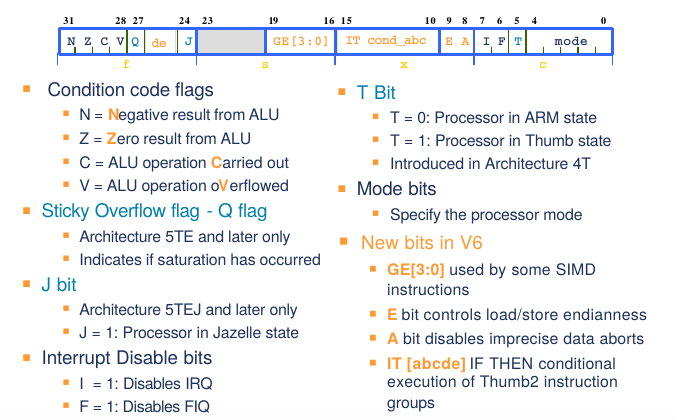
\includegraphics[width=.77\textwidth]{cpsr.pdf}
 \end{textblock*}
\end{frame}

\begin{frame}{Modos de operación}
 \begin{textblock*}{\textwidth}(.3cm,1.2cm) 
  \begin{scriptsize}
   \begin{center}
    \begin{tikzpicture}
     \node (tbl) { 
      \rowcolors[]{1}{}{gray!5}
      \begin{tabularx}{.59\textwidth}{l c c c}
       \textbf{\color{white} Modo} & \textbf{\color{white} Mnemónico} & \textbf{ \color{white} Privilegiado} & \textbf{ \color{white} CPSR[4:0]}\\
       Abort & abt & si & 10111\\
       Fast interrupt request & fiq & si & 10001\\
       Interrupt request & irq & si & 10010\\
       Supervisor & svc & si & 10011\\
       System & sys & si & 11111\\
       Undefined & und & si & 11011\\
       User & usr & no & 10000\\
      \end{tabularx}
     };
     \begin{pgfonlayer}{background}
      \draw[rounded corners,top color=red,bottom color=black,draw=white] ($(tbl.north west)+(0.14,0)$) rectangle ($(tbl.north east)-(0.13,0.45)$);
      \draw[rounded corners,top color=white,bottom color=black, middle color=red,draw=blue!20] ($(tbl.south west)+(0.12,0.5)$) rectangle ($(tbl.south east)-(0.12,0)$);
      \draw[top color=blue!1,bottom color=blue!20,draw=white] ($(tbl.north east)-(0.13,0.6)$) rectangle ($(tbl.south west)+(0.13,0.2)$);
     \end{pgfonlayer}
    \end{tikzpicture}
   \end{center}
  \end{scriptsize}
 \end{textblock*}
 \begin{textblock*}{\textwidth}(.3cm,5.2cm) 
  \begin{block}<2->{} \justifying
   Puede verse que excepto User el resto de los modos es Privilegiado. Lo cual significa que el kernel de un Sistema Operativo para un sistema basado en procesadores de ARM, se encargará de incluir todo el código que ejecute en estos modos.\\
   Las tareas y procesos por otra parte, ejecutarán en Modo User.
  \end{block}
 \end{textblock*}
\end{frame}

\begin{frame}{Vector de Interrupciones}
 \begin{textblock*}{\textwidth}(.3cm,.8cm)
  \begin{scriptsize}
   \begin{center}
    \begin{tikzpicture}
     \node (tbl) { 
      \rowcolors[]{1}{}{gray!5}
      \begin{tabularx}{.65\textwidth}{l c c c}
       \textbf{\color{white} Excepción/Interrupción} & \textbf{\color{white} Mnemónico} & \textbf{ \color{white}Dirección} & \textbf{ \color{white} Dirección Alta}\\
       Reset & RESET & 0x00000000 & 0xffff0000\\
       Undefined instruction & UNDEF & 0x00000004 & 0xffff0004\\
       Software interrupt & SWI & 0x00000008 & 0xffff0008\\
       Prefetch abort & PABT & 0x0000000c & 0xffff000c\\
       Data abort & DABT & 0x00000010 & 0xffff0010\\
       Reserved & - & 0x00000014 & 0xffff0014\\
       Interrupt request & IRQ & 0x00000018 & 0xffff0018\\
       Fast interrupt request & FIQ & 0x0000001c & 0xffff001c\\
      \end{tabularx}
     };
     \begin{pgfonlayer}{background}
      \draw[rounded corners,top color=red,bottom color=black,draw=white] ($(tbl.north west)+(0.14,0)$) rectangle ($(tbl.north east)-(0.13,0.45)$);
      \draw[rounded corners,top color=white,bottom color=black, middle color=red,draw=blue!20] ($(tbl.south west)+(0.12,0.5)$) rectangle ($(tbl.south east)-(0.12,0)$);
      \draw[top color=blue!1,bottom color=blue!20,draw=white] ($(tbl.north east)-(0.13,0.6)$) rectangle ($(tbl.south west)+(0.13,0.2)$);
     \end{pgfonlayer}
    \end{tikzpicture}
   \end{center}
  \end{scriptsize}
 \end{textblock*}
 \begin{textblock*}{.5\textwidth}(.3cm,4.4cm)
  \only<2>{\includegraphics[width=.85\textwidth]{chmode-layer1.pdf}}
  \only<3>{\includegraphics[width=.85\textwidth]{chmode-layer2.pdf}}
  \only<4>{\includegraphics[width=.85\textwidth]{chmode-layer3.pdf}}
  \only<5>{\includegraphics[width=.85\textwidth]{chmode-layer4.pdf}}
  \only<6>{\includegraphics[width=.85\textwidth]{chmode-layer5.pdf}}
  \only<7>{\includegraphics[width=.85\textwidth]{chmode-layer6.pdf}}
  \only<8>{\includegraphics[width=.85\textwidth]{chmode-layer7.pdf}}
 \end{textblock*}
 \begin{textblock*}{.5\textwidth}(.45\textwidth ,4.4cm)
  \begin{itemize} \justifying
   \item <4->Al generarse la interrupción se salva \textbf{\texttt{CPSR}} en el \texttt{\textbf{SPSR}} del modo al que se pasa.
   \item <5->Siempre se usa \textbf{\texttt{CPSR}}. Solo cambia \textbf{\texttt{CPSR[4:0]}}
   \item <6->LR=Dirección de retorno.
   \item <7->Al saltar desde el Vector de Interrupciones el \textbf{\texttt{PC}} toma la dirección destino.
  \end{itemize}
 \end{textblock*}
\end{frame}

\begin{frame}{Tabla de vectores}
 \begin{textblock*}{\textwidth}(.3cm,1.2cm)
  \begin{itemize}[<+(1)->] \justifying \parskip 0.3cm
   \item Por default se ubica en la dirección 0. 
   \item CORTEX A y R permiten ubicarla en 0xFFFF0000. Puede resultar mas práctico cuando se tiene un sistema operativo.
   \item Cada entrada puede contener una instrucción que genere un branch. Posibilidades:
   \begin{itemize}[<+(1)->] \justifying \parskip 0.3cm
    \item \texttt{b \#address} (salto relativo al \texttt{\textbf{PC}})
    \item \texttt{ldr pc,[pc, \#offset]} 
    \item \texttt{mov pc, \#immediate} (dato inmediato al PC rotado a derecha)
   \end{itemize}
  \end{itemize}
 \end{textblock*}
\end{frame}

\begin{frame}{Prioridad de las Excepciones}
 \begin{textblock*}{\textwidth}(.3cm,1.0cm)
  \begin{scriptsize}
   \begin{center}
    \begin{tikzpicture}
     \node (tbl) { 
      \rowcolors[]{1}{}{gray!5}
      \begin{tabularx}{.579\textwidth}{l c c c}
       \textbf{\color{white} Excepción} & \textbf{\color{white} Prioridad} & \textbf{ \color{white}Bit CPSR[I]} & \textbf{ \color{white} Bit CPSR[F]}\\
       Reset & 1 & 1 & 1\\
       Data abort & 2 & 1 & -\\
       Fast interrupt request & 3 & 1 & 1\\
       Interrupt request & 4 & 1 & -\\
       Prefetch abort & 5 & 1 & -\\
       Software interrupt & 6 & 1 & -\\
       Undefined instruction & 6 & 1 & -\\
      \end{tabularx}
     };
     \begin{pgfonlayer}{background}
      \draw[rounded corners,top color=red,bottom color=black,draw=white] ($(tbl.north west)+(0.14,0)$) rectangle ($(tbl.north east)-(0.13,0.45)$);
      \draw[rounded corners,top color=white,bottom color=black, middle color=red,draw=blue!20] ($(tbl.south west)+(0.12,0.5)$) rectangle ($(tbl.south east)-(0.12,0)$);
      \draw[top color=blue!1,bottom color=blue!20,draw=white] ($(tbl.north east)-(0.13,0.6)$) rectangle ($(tbl.south west)+(0.13,0.2)$);
     \end{pgfonlayer}
    \end{tikzpicture}
   \end{center}
  \end{scriptsize}
 \end{textblock*}
 \begin{textblock*}{\textwidth}(.3cm,4.4cm)
  \begin{itemize}[<+(1)->]\justifying
   \item Esta tabla define en que orden se atienden las excepciones en caso de simultaneidad.
   \item \textbf{\textit{Reset}} tiene máxima preeminencia por sobre las demás. 
   \item En un \textit{\textbf{Reset}} debe inicializarse el sistema completo, habilitar la memoria los caches y armar el vector de excepciones antes de habilitar \textbf{\textit{IRQ}} y \textit{\textbf{FIQ}}.
   \item Las primeras instrucciones de este handler deben garantizar que no ocurra ninguna excepción. Por eso deben estar deshabilitadas \textbf{\textit{IRQ}} y \textbf{\textit{FIQ}} (Flags \textbf{I} y \textbf{F} en '1').
  \end{itemize}
 \end{textblock*}
\end{frame}

\begin{frame}{Prioridad de las Excepciones}
 \begin{textblock*}{\textwidth}(.3cm,1.2cm)
  \begin{itemize}[<+->]\justifying \parskip 0.3cm
   \item \textbf{\textit{Data Abort}} es generada por la MMU. Escenarios mas comunes:
   \begin{itemize} \justifying \parskip 0.3cm
    \item Cuando se intenta acceder a una dirección de memoria inválida (si no hay memoria física asignada a esa dirección de memoria).
    \item Cuando se intenta acceder a una dirección de memoria para la cual no se dispone de los permisos necesarios.
   \end{itemize}
   \item Sin embargo no hay problemas en suspender la atención de un \textbf{\textit{Data Abort}} para vectorizar el handler de una \textit{\textbf{FIQ}}. Eventualmente una vez que termina el handler de \textbf{\textit{FIQ}} se retorna al de \textbf{\textit{Data Abort}} y se continúa con su resolución.
   \item Decimos que \textbf{\textit{Data Abort}} soporta anidamiento con \textit{\textbf{FIQ}}.
  \end{itemize}
 \end{textblock*}
\end{frame}

\begin{frame}{Prioridad de las Excepciones}
 \begin{textblock*}{\textwidth}(.3cm,1.2cm)
  \begin{itemize}[<+->] \justifying \parskip 0.3cm
   \item \textbf{\textit{FIQ}}, se produce cuando un periférico lleva el terminal \textit{\textbf{FIQ}} del procesador al estado \textit{nFIQ}.
   \item El core deshabilita \textbf{\textit{FIQ}} e \textit{\textbf{IRQ}} cuando vectoriza \textbf{\textit{FIQ}}.
   \item \textbf{\textit{IRQ}}, se produce cuando un periférico lleva el terminal \textit{\textbf{IRQ}} del procesador al estado \textit{nIRQ}.
   \item El core deshabilita \textit{\textbf{IRQ}} cuando la vectoriza.
  \end{itemize}
 \end{textblock*}
\end{frame}

\begin{frame}{Prioridad de las Excepciones}
 \begin{textblock*}{\textwidth}(.3cm,1.2cm)
  \begin{itemize}[<+->] \justifying \parskip 0.3cm
   \item Se genera \textit{\textbf{Prefetch Abort}} cuando se intenta un Fetch de una instrucción en una dirección inválida de memoria.
   \item Esta excepción se genera cuando la instrucción responsable del Fallo ingresa a la etapa de ejecución del pipeline, siempre que no se hayan activado en el transcurso \textbf{\textit{FIQ}}, y/o \textit{\textbf{IRQ}} (recordar el caracter asincrónico y no determinístico de las interrupciones de hardware).
   Si esto hubiese ocurrido se atenderá la interrupción o ambas interrupciones (según corresponda) en el orden de prioridad establecido.
   \item Cuando se vectoriza \textbf{\textit{Prefetch Abort}}, se deshabilita \textbf{\textit{IRQ}}. 
   \item El handler de \textit{\textbf{Prefetch Abort}}, se suspende si ingresa \textbf{\textit{FIQ}}, o\textbf{\textit{IRQ}}, si se habilitó en algún momento durante la ejecución del handler. 
  \end{itemize}
 \end{textblock*}
\end{frame}

\begin{frame}{Prioridad en las Excepciones}
 \begin{textblock*}{\textwidth}(.3cm,1.2cm)
  \begin{itemize}[<+->] \justifying \parskip 0.3cm
   \item \textbf{\textit{SWI}} se genera cuando se ejecuta la Instrucción \textbf{\textit{SWI}} o \textbf{\textit{SVC}} (\textbf{\textit{SWI}} sigue implementada pero es considerada obsoleta por ARM desde 2007).
   \item Esta instrucción se ejecuta en código Modo User. 
   \item Al ingresar al handler, el procesador establece en el registro CPSR el Modo Supervisor.
  \end{itemize}
 \end{textblock*}
\end{frame}

\begin{frame}{Prioridad en las Excepciones}
 \begin{textblock*}{\textwidth}(.3cm,1.2cm)
  \begin{itemize}[<+->] \justifying \parskip 0.3cm
   \item \textbf{\textit{Undefined Instruction}} se genera en la fase de ejecución del pipeline cuando la instrucción no corresponde al set de instrucciones ARM Thumb o Thumb2 y no hay coprocesadores disponibles y si los hay tampoco corresponde a sus instrucciones.
   \item \textbf{\textit{Undefined Instruction}} y \textbf{\textit{SWI}} nunca pueden por razones obvias ocurrir al mismo tiempo. Por eso tienen la misma prioridad.
  \end{itemize}
 \end{textblock*}
\end{frame}

\begin{frame}{Dirección de retorno. Valores del Link Register}
 \begin{textblock*}{\textwidth}(.3cm,.9cm)
  \begin{scriptsize}
   \begin{center}
    \begin{tikzpicture}
     \node (tbl) { 
      \rowcolors[]{1}{}{gray!5}
      \begin{tabularx}{.78\textwidth}{l c l}
       \textbf{\color{white} Excepción} & \textbf{\color{white} Dirección} & \textbf{ \color{white}Uso}\\
       Reset & - & Es un Reset. No está definido\\
       Data abort & lr - 8 & Apunta a la instrucción que causó el Abort\\
       Fast interrupt request & lr - 4 & Retorna a la instrucción siguiente a la que recibió FIQ\\
       Interrupt request & lr - 4 & Retorna a la instrucción siguiente a la que recibió IRQ\\
       Prefetch abort & lr - 4 & Retorna a la instrucción que recibió Prefetch Abort\\
       Software interrupt & lr & Regresa a la instrucción siguiente a SWI\\
       Undefined instruction & lr & Regresa a la instrucción siguiente a la no definida\\
      \end{tabularx}
     };
     \begin{pgfonlayer}{background}
      \draw[rounded corners,top color=red,bottom color=black,draw=white] ($(tbl.north west)+(0.14,0)$) rectangle ($(tbl.north east)-(0.13,0.45)$);
      \draw[rounded corners,top color=white,bottom color=black, middle color=red,draw=blue!20] ($(tbl.south west)+(0.12,0.5)$) rectangle ($(tbl.south east)-(0.12,0)$);
      \draw[top color=blue!1,bottom color=blue!20,draw=white] ($(tbl.north east)-(0.13,0.6)$) rectangle ($(tbl.south west)+(0.13,0.2)$);
     \end{pgfonlayer}
    \end{tikzpicture}
   \end{center}
  \end{scriptsize}
  \vspace{-0.4cm}
  \begin{itemize}[<+(1)->]\justifying
   \item Tener presente que todas las excepciones ocurren durante la etapa de ejecución de la instrucción en el pipeline
   \item Lo mismo las Interrupciones de Hardware. Independientemente de cuando ingresan, se atienden luego de completar la ejecución de la instrucción en curso.
   \item Como el pipeline es de tres etapas, y el tamaño de ejecución es fijo, en la fase de ejecución en modo ARM el registro \textit{\textbf{PC}}, está posicionado para fetchear dos instrucciones mas adelante.
   \item Por ello en \textbf{\textit{LR}} se guarda el valor actual del \textbf{\textit{PC}} mas 8.
  \end{itemize}
 \end{textblock*}
\end{frame}

\begin{frame}{Dirección de retorno en LR de Data Abort.}
 \begin{textblock*}{\textwidth}(.3cm,1.2cm)
  \centering 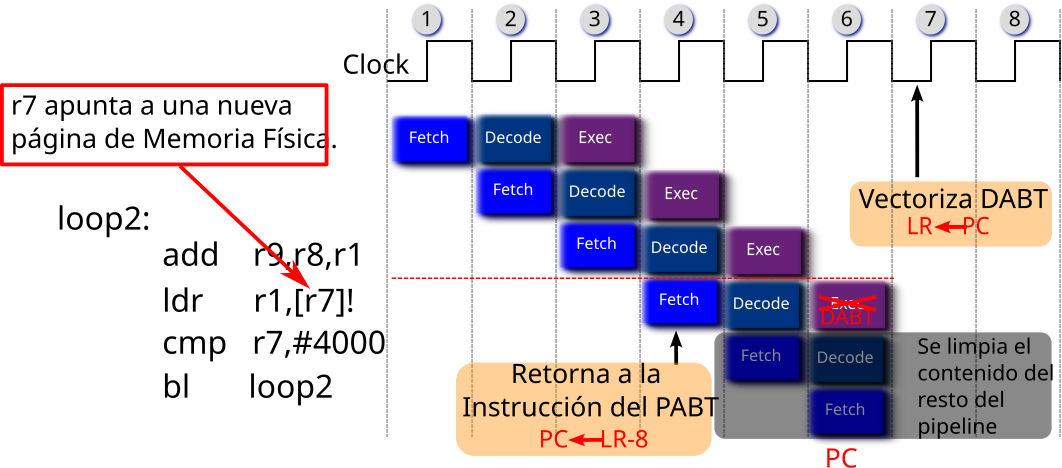
\includegraphics[width=\textwidth]{ARM-pipeline-DABT.pdf}
 \end{textblock*}
\end{frame}

\begin{frame}{Dirección de retorno en LR de Prefetch Abort.}
 \begin{textblock*}{\textwidth}(.3cm,1.2cm)
  \centering 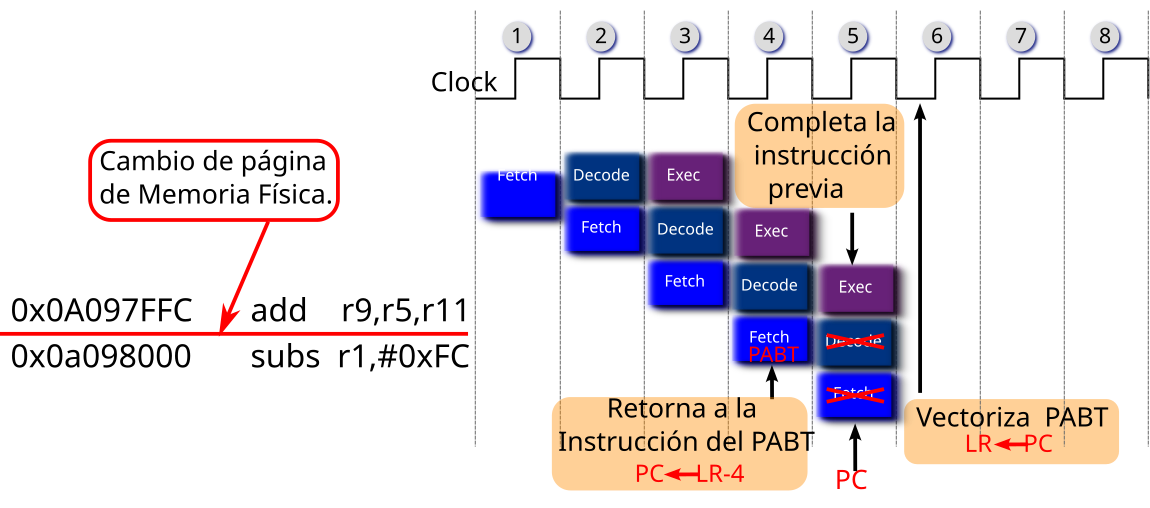
\includegraphics[width=\textwidth]{ARM-pipeline-PABT.pdf}
 \end{textblock*}
\end{frame}

\begin{frame}{Dirección de retorno en LR de SVC o Undef.}
 \begin{textblock*}{\textwidth}(.3cm,1.2cm)
  \centering 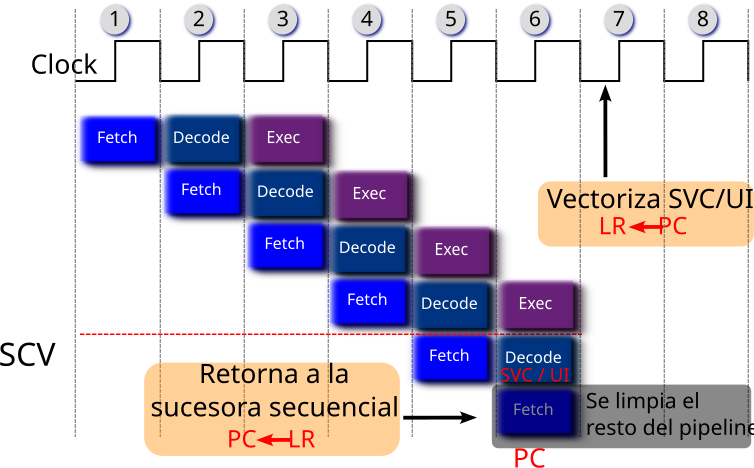
\includegraphics[width=0.7\textwidth]{ARM-pipeline-SVC-UI.pdf}
 \end{textblock*}
\end{frame}
 
\begin{frame}[t,fragile]{Ejemplos de Código de retorno para \textbf{\texttt{IRQ}} y \texttt{\textbf{FIQ}}}
 \begin{textblock*}{\textwidth}(.3cm,.9cm)
  \lstset{language=[ARM]Assembler,basicstyle=\scriptsize,}
  \begin{lstlisting}[escapechar=\@,numbers=none, frame=single, xleftmargin=20pt, xrightmargin=0pt,]
handler:
    /*handler code*/
    ...
    subs pc, r14, #4        /*pc=r14-4*/
---------------------------------------------------------------------
handler:
    sub  r14, r14, #4       /*r14-=4*/
    ...
    /*handler code*/
    ...
    movs pc, r14            /*return*/
---------------------------------------------------------------------
handler:
    sub   r14, r14, #4      /*r14-=4*/
    stmfd r13!,{r0-r3, r14} /*Almacena contexto. (PUSH) r13=sp.*/
    ...                     /*FD=Full Descending. Decrement Before.*/
    /*handler code*/
    ...
    ldmfd r13!,{r0-r3, pc}  /*Recupera Contexto. (POP) r13=sp. LR->PC.*/
                            /*FD=Full Descending. Increment After.*/
  \end{lstlisting}
 \end{textblock*}
\end{frame}

\subsection{Interrupciones}
\begin{frame}{Diseño del Sistema de Interrupciones}
 \begin{textblock*}{\textwidth}(.3cm,1.2cm)
  \begin{block}<1->{Guidelines para el diseñador de un sistema embebido}
   \begin{enumerate}[<+(1)->] \justifying \parskip 0.3cm
    \item Seleccionar o diseñar un controlador de interrupciones adecuado para colectar las diferentes fuentes de interrupción de los diversos dispositivos de E/S, priorizarlas adecuadamente, y distribuirlas hacia IRQ o FIQ, y manejar un sistema de habilitación / deshabilitación particular para cada una.
    \begin{itemize} \justifying \parskip 0.3cm
     \item Las interrupciones de propósito general van a IRQ (Ejemplo un timer que obra como base de tiempos para cambios de tarea)
     \item Las interrupciones en donde es crítico el tiempo de respuesta van a FIQ. Ejemplo: DMA.
    \end{itemize}
    \item Diseñar un sistema de software compuesto por los diferentes handlers de cada dispositivo, acorde con los requerimientos de hardware.
   \end{enumerate}
  \end{block}
 \end{textblock*}
\end{frame}

\begin{frame}{Interrupt Latency}
 \begin{textblock*}{\textwidth}(.3cm,1.2cm)
  \begin{itemize}[<+(1)->] \justifying \parskip 0.3cm
   \item Si lo que estamos diseñando es un sistema event driven, entonces la madre de todas las batallas se llama  \textit{\textquotedblleft Interrupt Latency"}.
   \item \textit{Latency} proviene de Late. Podríamos asemejarlo a retardo.
   \item Sin embargo en argento básico ... se dice latencia (como si latiera\dots)
   \item Nuestro trabajo cuando hay múltiples fuentes de interrupción es encontrar el mejor sistema de gestión de interrupciones que minimice este retardo
  \end{itemize}
 \end{textblock*}
\end{frame}

\begin{frame}{Abordajes para mínimo Interrupt Latency}
 \begin{textblock*}{\textwidth}(.3cm,1.2cm)
  \begin{block}<1->{Anidamiento :}\justifying
   Consiste en permitir que una interrupción pueda ser suspendida cuando otra requiere servicio de modo que ésta no deba esperar que se complete la anterior. \newline
   Funciona muy bien en sistemas de periféricos de similar complejidad y donde todos juegan con un sistema de prioridades mas o menos uniforme (plano)
  \end{block} 
  \begin{block}<2->{Priorización:}\justifying
   Consiste en asignar una jerarquía basada en prioridades de modo que cada interrupción pueda anidar el procesamiento únicamente de interrupciones de mayor prioridad.

   Si los dispositivos tienen igual o menos prioridad no se cursa la nueva interrupción hasta que no finalice la interrupción en curso, así la nueva se encuentre habilitada.
  \end{block}
 \end{textblock*}
\end{frame}

\begin{frame}{Secuencia de Atención de IRQ}
 \begin{textblock*}{\textwidth}(.3cm,1.2cm)
  \only<1>{\centering\includegraphics[width=.7\textwidth]{chmode-layer1.pdf}\\}
  \only<2>{\centering\includegraphics[width=.7\textwidth]{chmode-layer2.pdf}\\}
  \only<3>{\centering\includegraphics[width=.7\textwidth]{chmode-layer3.pdf}\\}
  \only<4>{\centering\includegraphics[width=.7\textwidth]{chmode-layer4.pdf}\\}
  \only<5>{\centering\includegraphics[width=.7\textwidth]{chmode-layer5.pdf}\\}
  \only<6>{\centering\includegraphics[width=.7\textwidth]{chmode-layer6.pdf}\\}
  \only<7>{\centering\includegraphics[width=.7\textwidth]{chmode-layer7.pdf}\\}
 \end{textblock*}
\end{frame}

\begin{frame}{Secuencia de Atención de FIQ}
 \begin{textblock*}{\textwidth}(.3cm,1.2cm)
  \only<1>{\centering\includegraphics[width=.7\textwidth]{chmodeF-layer1.pdf}\\}
  \only<2>{\centering\includegraphics[width=.7\textwidth]{chmodeF-layer2.pdf}\\}
  \only<3>{\centering\includegraphics[width=.7\textwidth]{chmodeF-layer3.pdf}\\}
  \only<4>{\centering\includegraphics[width=.7\textwidth]{chmodeF-layer4.pdf}\\}
  \only<5>{\centering\includegraphics[width=.7\textwidth]{chmodeF-layer5.pdf}\\}
  \only<6>{\centering\includegraphics[width=.7\textwidth]{chmodeF-layer6.pdf}\\}
  \only<7>{\centering\includegraphics[width=.7\textwidth]{chmodeF-layer7.pdf}\\}
 \end{textblock*}
\end{frame}

\begin{frame}[fragile]{Habilitación de IRQ y FIQ}
 \begin{textblock*}{\textwidth}(.3cm,1.2cm)
Para habilitación I=0 y F=0 
  \lstset{language=[ARM]Assembler,basicstyle=\scriptsize,}
  \begin{lstlisting}[numbers=none, frame=single, xleftmargin=20pt, xrightmargin=0pt, escapechar=\@,]
IRQ_Enable:
  mrs r1,cpsr     //mrs mover a registro core desde registro de sistema o coprocesador
  bic r1,r1,#0x80 //Bit Clear. Limpia en el registro los bits seteados en el valor inmediato
  msr cpsr,r1     //msr, operacion inversa de mrs
  
FIQ_Enable:
  mrs r1,cpsr
  bic r1,r1,#0x40
  msr cpsr,r1
  \end{lstlisting}
 \end{textblock*}
\end{frame}

\begin{frame}[fragile]{Habilitación - Deshabilitación de IRQ y FIQ}
 \begin{textblock*}{\textwidth}(.3cm,1.2cm)
Código para deshabilitación
  \lstset{language=[ARM]Assembler,basicstyle=\scriptsize,}
  \begin{lstlisting}[numbers=none, frame=single, xleftmargin=20pt, xrightmargin=0pt,]
IRQ_Disable:
  mrs r1,cpsr     //mrs mover a registro core desde registro de sistema o coprocesador
  orr r1,r1,#0x80 //Orr. Setea en el registro los bits seteados en el valor inmediato
  msr cpsr,r1     //msr, operacion inversa de mrs
    
FIQ_Disable
  mrs r1,cpsr
  orr r1,r1,#0x40
  msr cpsr,r1
  \end{lstlisting}
 \end{textblock*}
\end{frame}

%%%%%%%%%%%%%%%%%%%%%%%%%%%%%%%%%%%%%%%%%%%%%%%%%%%%%%%%%%%%%%%%%%%%%%%%%%%%%%%%%%%%%%%%%%%%%%%%%%%%%%%%%%%%%%%%%%%%%%%%%%%%%%%%%%
%Para completar %%%%%%%%
\subsection{Ejemplo práctico de controlador de Interrupciones}
\begin{frame}{SOC SITARA AM335x: Controlador de Interrupciones}
 \begin{textblock*}{.36\textwidth}(.3cm,1.2cm)
  \centering 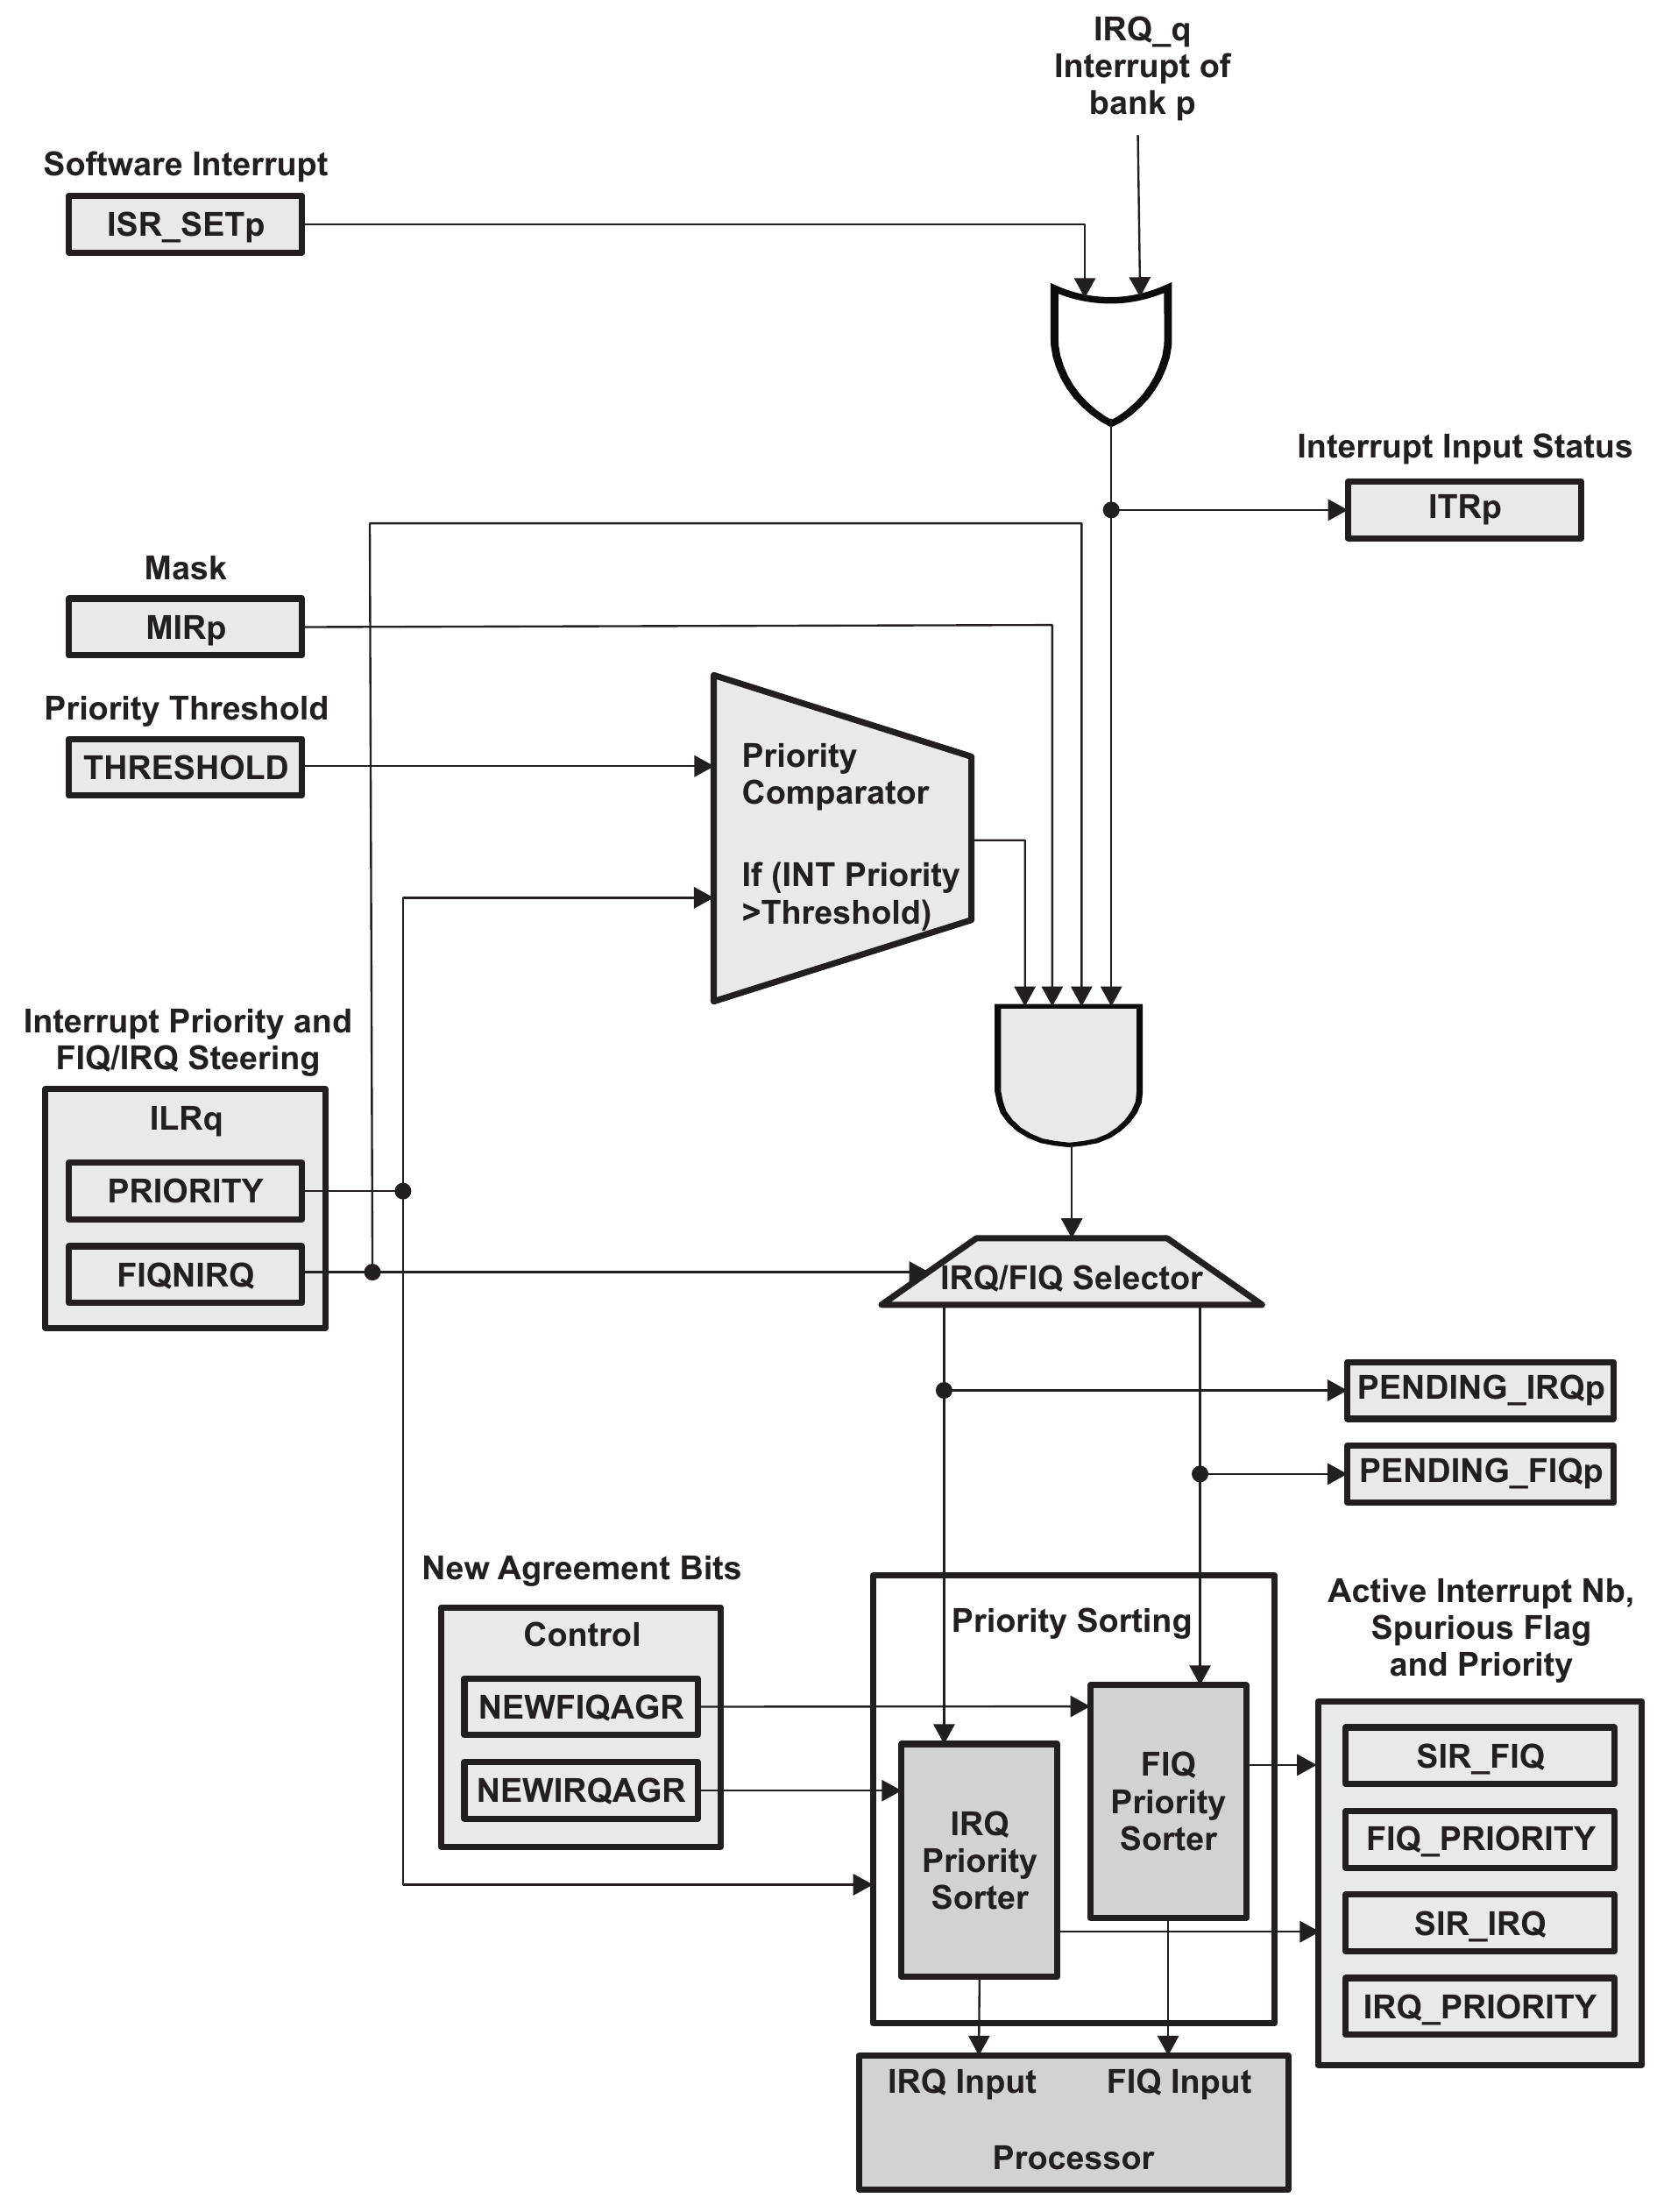
\includegraphics[width=\textwidth]{AM335x-InterruptController.png}
 \end{textblock*}
 \begin{textblock*}{.67\textwidth}(.36\textwidth,1.2cm)
  \begin{itemize}[<+(1)->] \justifying
   \item ARM especifica un Controlador de Interrupciones Genérico (GIC). Sin embargo no lo impone como Controlador de Interrupciones para sus cores.
   \item Esa decisión de diseño favorece a los fabricantes que pueden utilizar sus propios controladores en caso que tengan diseños probados.
   \item Texas Instruments, produce el SoC SITARA 3358, basado en un core con un procesador Cortex-A8, con un sistema de split cache L1 \SI{32}{\kibi\byte} para código y otro para datos, y cache L2 de \SI{256}{\kibi\byte}.
   \item El SITARA 3358 viene con un Controlador de interrupciones como el de la Figura que es un diseño adaptado de los controladores de interrupciones presente en los modelos anteriores de Texas para otros cores propios.
  \end{itemize}  
 \end{textblock*}
\end{frame}

\begin{frame}{SOC SITARA AM335x: Controlador de Interrupciones}
  \begin{textblock*}{.36\textwidth}(.3cm,1.2cm)
   \centering 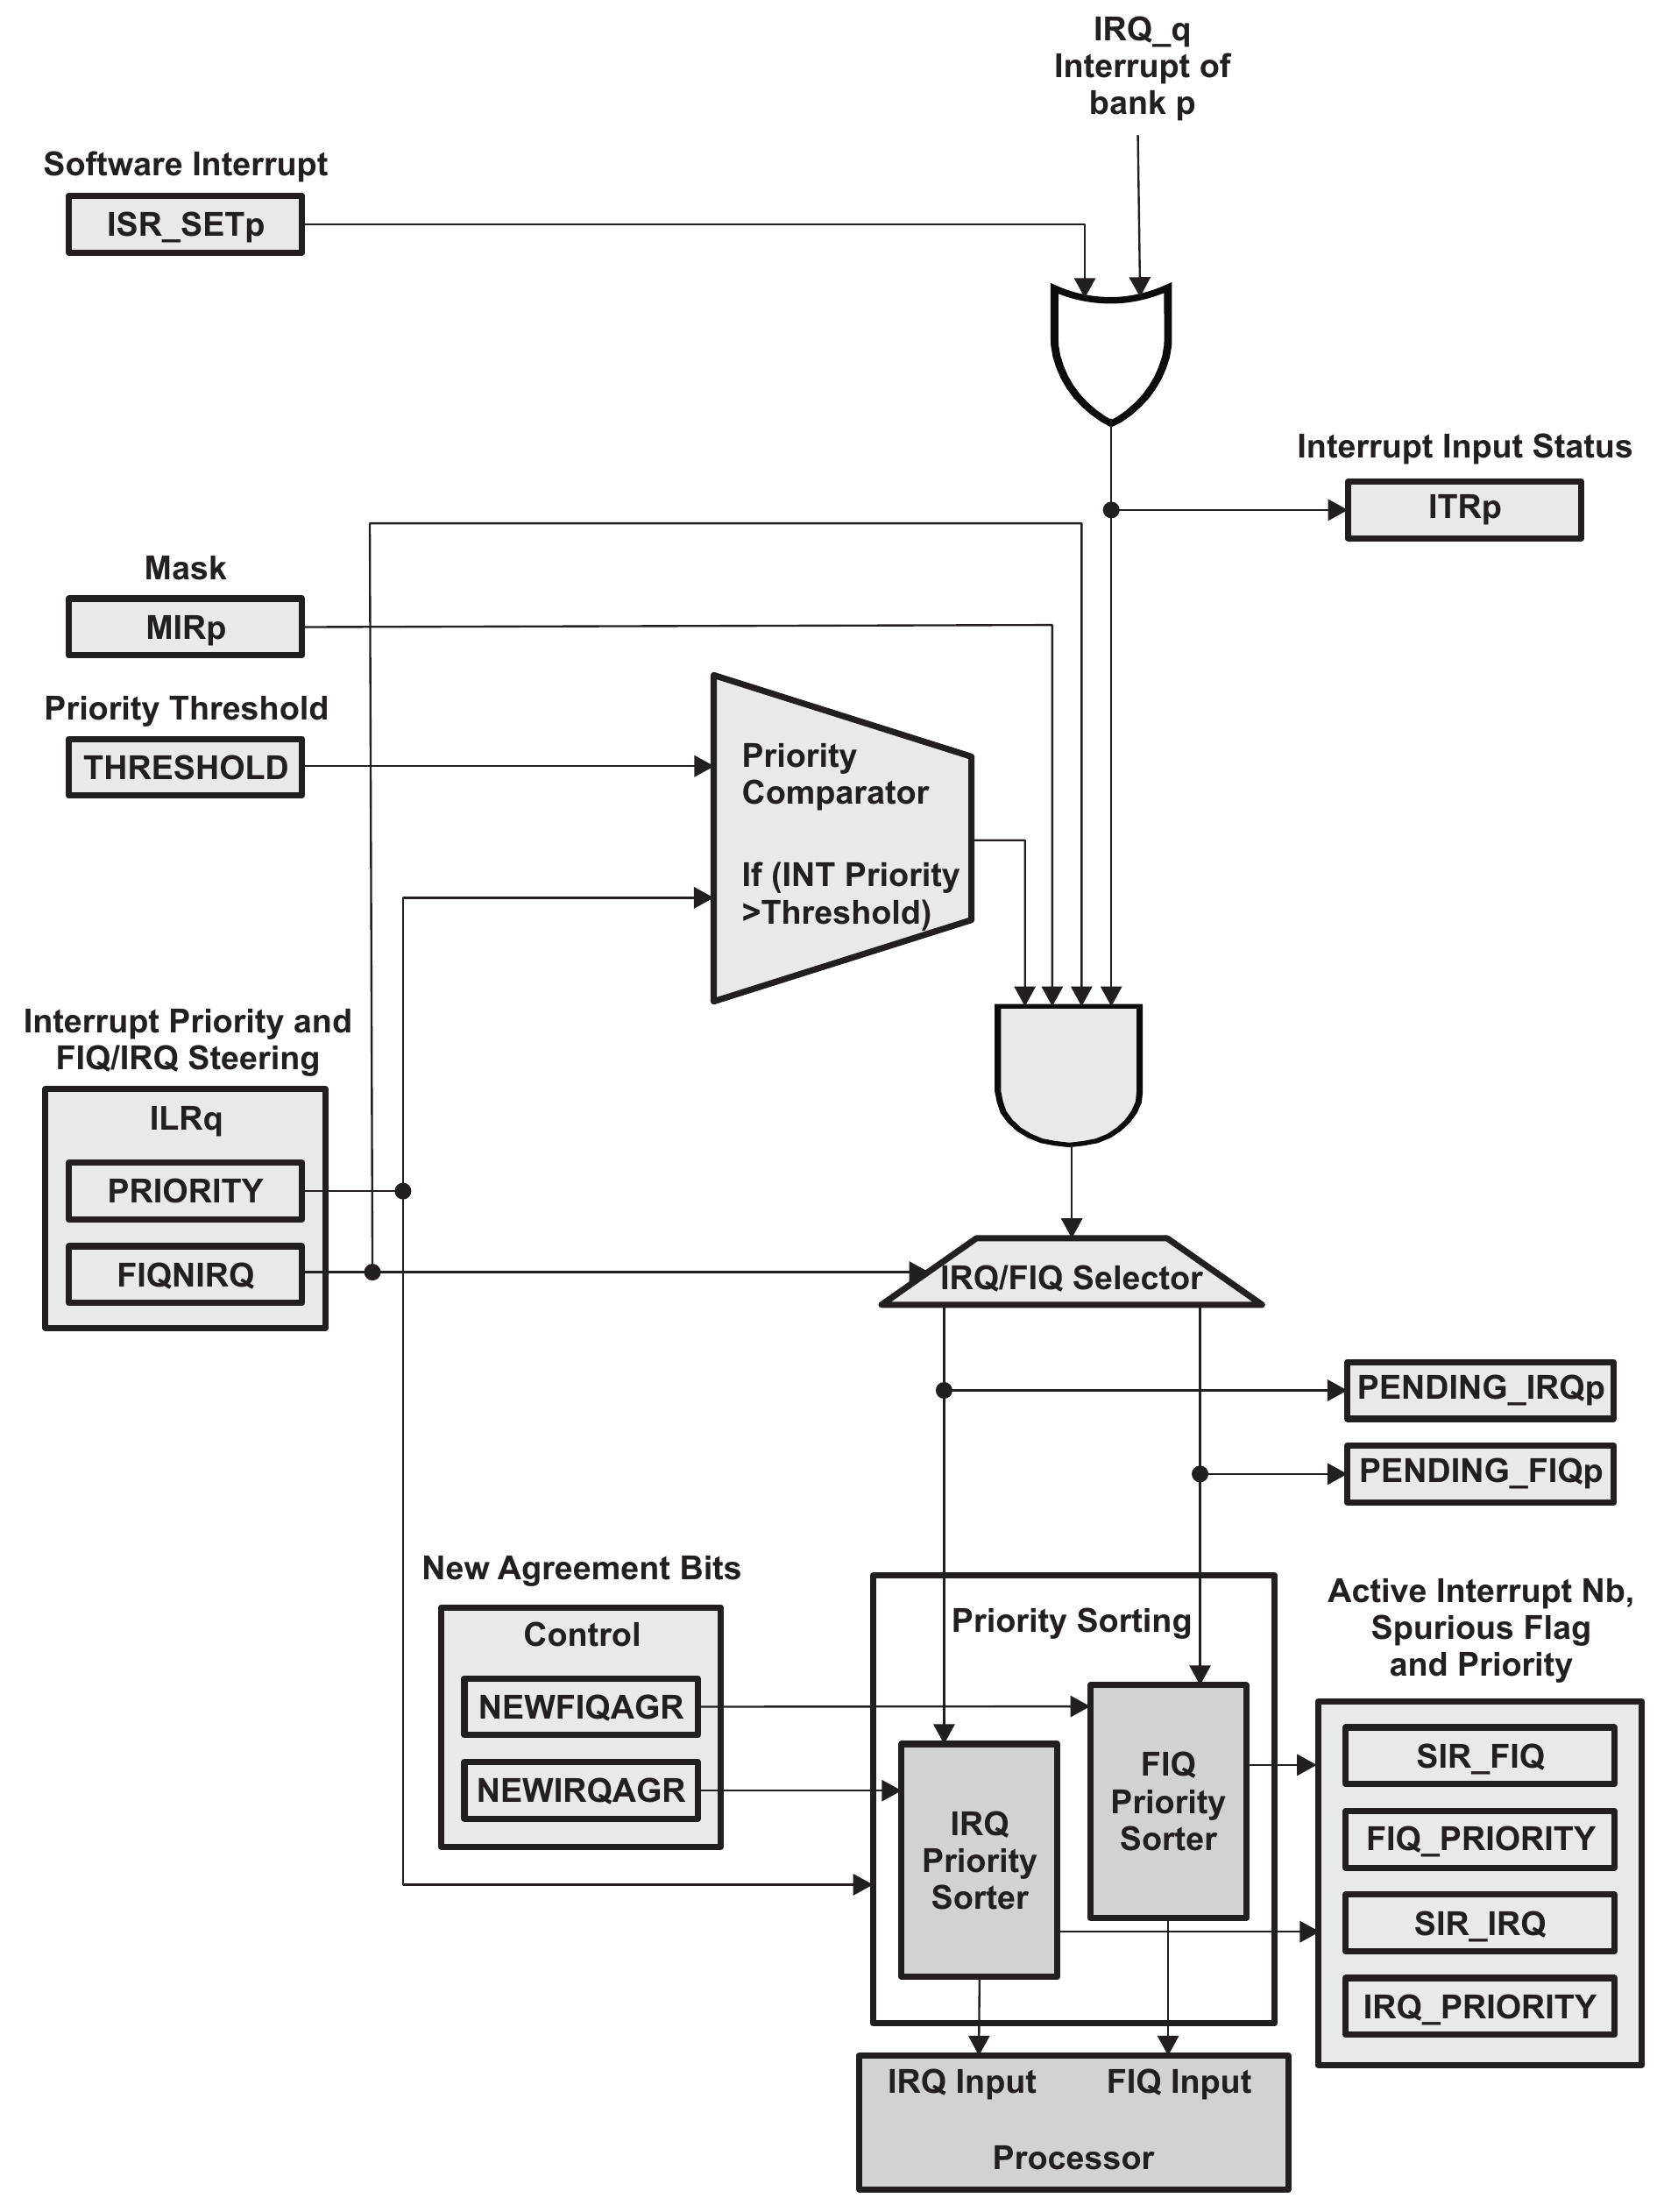
\includegraphics[width=\textwidth]{AM335x-InterruptController.png}
  \end{textblock*}
  \begin{textblock*}{.67\textwidth}(.36\textwidth,1.2cm)
   \begin{itemize}[<+->] \justifying
    \item Soporta 128 fuentes diferentes de interrupción. 
    \item La primer consecuencia es que al ser un procesador de Aplicación Texas decide no dar soporte a FIQ. 
    \item Permite definir máscaras individuales para las diferentes fuentes de interrupción.
    \item Permite definir 128 umbrales de prioridad. 
    \item Soporta pre emption
    \item Al ser propietario el firmware que desarrollamos solo se aplica en los SoC de Texas.
    \item Ventajas para los fabricantes pero desventajas para los desarrolladores
   \end{itemize}  
  \end{textblock*}
 \end{frame}
 
 %%%%%%%%%%%%%%%%%%%%%%%%%%%%%%%%%%%%%%%%%%%%%%%%%%%%%%%%%%%%%%%%%%%%%%%%%%%%%%%%%%%%%%%%%%%%%%%%%%%%%%%%%%%%%%%%%%%%%%%%%%%%%%%%%%

\section{Interrupciones de Hardware}
\subsection{Características y Modos de trabajo}
\begin{frame}{ARMv7 Interrupciones Externas (hardware)}
 \begin{textblock*}{\textwidth}(0.4cm,1.2cm)
  \begin{itemize}[<+(1)->]\justifying 
   \item El Controlador de Interrupciones de un core ARMv7 puede diseñarse en forma específica para el SoC, o ser una implementación de la arquitectura ARM Generic Interrupt Controller (GIC).
   \item Cualquier procesador de ARM tiene dos líneas de entrada para recibir requerimientos de interrupción desde dispositivos externos: \textbf{\texttt{IRQ}} y \texttt{\textbf{FIQ}}. Ambas activas bajas.
   \item Los requerimientos de interrupción que puede enviar la diversidad de dispositivos de E/S conectados al Core, finalmente deben ser mapeados en \textbf{\texttt{IRQ}} o \texttt{\textbf{FIQ}}.
   \item Antes del Controlador de Interrupciones...
   \item Cada entrada responderá al requerimiento siempre que los bits de deshabilitación \textbf{\texttt{CPSR.I}} y \textbf{\texttt{CPSR.F}} estén en '0'.
  \end{itemize}
  \only<7->{\vspace{-0.3cm} \begin{center}
\includegraphics[width=0.9\textwidth]{cpsr-bits-IF.pdf}\end{center}}
 \end{textblock*}
\end{frame}

\begin{frame}[fragile]{ARMv7 Interrupciones Externas (hardware)}
 \begin{textblock*}{\textwidth}(0.4cm,1.2cm) \justifying
La instrucción \textbf{\texttt{CPS}} (Change Processor State) permite manejar de manera simple estos dos bits, junto con el bit \textit{Abort Enable} \textbf{\texttt{CPSR.A}}, y también al mismo tiempo establecer el Modo del procesador.

Sintaxis:\vspace{-0.3cm}
   \begin{lstlisting}[basicstyle=\scriptsize,escapechar=\@,numbers=none, frame=single, xleftmargin=20pt, xrightmargin=0pt,]
CPSeffect iflags{, #mode}
CPS #mode
   \end{lstlisting}
\vspace{-0.3cm} \textit{effect}:  Define la operación. \texttt{\textbf{IE}}: Interrupt/Abort Enable, o \texttt{\textbf{ID}}: Interrupt/Abort Disable

\textit{iflags}: Define el objeto de la operación \texttt{\textbf{a}}: aborts imprecisos, \texttt{\textbf{i}}: interrupciones \texttt{\textbf{IRQ}}, o \texttt{\textbf{f}}: Interrupciones \texttt{\textbf{FIQ}}

Ejemplos:\vspace{-0.3cm}
   \begin{lstlisting}[basicstyle=\scriptsize,escapechar=\@,numbers=none, frame=single, xleftmargin=20pt, xrightmargin=0pt,]
CPSIE if      /*Habilita IRQ y FIQ.*/
CPSID a       /*Deshabilita aborts imprecisos.*/
CPSID ai, #17 /*Deshabilita aborts imprecisos e interrupciones, e ingresa a modo FIQ*/
CPS   #16     /*Entra a modo User*/
   \end{lstlisting}
 \end{textblock*}
\end{frame}

\subsection{Manejo de Múltiples Interrupciones}
\begin{frame}{Manejo de Interrupciones Simple}
 \begin{textblock*}{\textwidth}(0.4cm,1.5cm) \justifying
\only<2->{
  \begin{block}{Funcionamiento}\justifying
   Una vez que se produce un tipo de interrupción determinado, las demás interrupciones del mismo tipo se deshabilitan automáticamente, hasta que finalice la atención de la que está en curso. No hay priorización alguna.
  \end{block}
}
 \end{textblock*}
 \begin{textblock*}{\textwidth}(0.4cm,4.7cm) \justifying
\only<3->{
  \begin{block}{Características}\justifying
   No es apto para sistemas complejos, sino mas bien para probar preliminarmente algún handler critico no reentrante.
  \end{block}
}
 \end{textblock*}
\end{frame}

\begin{frame}{Manejo de Interrupciones Simple (IRQ)}
 \begin{textblock*}{0.65\textwidth}(0.4cm,1.1cm) 
  \begin{enumerate}[<+(1)->]\justifying
   \item \textbf{\texttt{PC}} \textrightarrow \texttt{\textbf{LR\_IRQ}}
   \item \textbf{\texttt{SPSR\_IRQ}} \textleftarrow \texttt{\textbf{CPSR}}
   \begin{enumerate}\justifying
    \item \textbf{\texttt{CPSR.Mode[4:0]}} \textleftarrow 10010
    \item \texttt{\textbf{CPSR.I}} \textleftarrow 1
   \end{enumerate}
   \item \textbf{\texttt{PC}} \textleftarrow Vector Table IRQ Entry
   \item Ejecuta la instrucción de la IRQ Entry (típicamente un salto)
   \item El handler salva en el stack (push) el/los registros que puedan ser alterados.
   \item Se ejecuta el core del handler.
   \item Restaura (pop) los registros apilados (observando el orden respecto del caracter LIFO de las pilas).
   \item Regresa: \textbf{\texttt{PC}} \textleftarrow \texttt{\textbf{LR\_IRQ}}, \newline \texttt{\textbf{CPSR}} \textleftarrow \textbf{\texttt{SPSR\_IRQ}}
  \end{enumerate}
 \end{textblock*}
 \begin{textblock*}{0.36\textwidth}(0.8cm+0.65\textwidth,1.0cm)
  \only<1>{\begin{center}\includegraphics[width=0.95\textwidth]{Vectoring-single-layer1.pdf}\end{center}}
  \only<2-6>{\begin{center}\includegraphics[width=0.95\textwidth]{Vectoring-single-layer2.pdf}\end{center}}
  \only<7>{\begin{center}\includegraphics[width=0.95\textwidth]{Vectoring-single-layer3.pdf}\end{center}}
  \only<8-10>{\begin{center}\includegraphics[width=0.95\textwidth]{Vectoring-single-layer4.pdf}\end{center}}
  \only<11>{\begin{center}\includegraphics[width=0.95\textwidth]{Vectoring-single-layer5.pdf}\end{center}}
 \end{textblock*}
\end{frame}

\begin{frame}[t]{Manejo de Interrupciones Simple (FIQ)}
 \begin{textblock*}{0.65\textwidth}(0.4cm,1.1cm) 
  \begin{enumerate}\justifying
   \item \textbf{\texttt{PC}} \textrightarrow \texttt{\textbf{LR\_FIQ}}
   \item \textbf{\texttt{SPSR\_FIQ}} \textleftarrow \texttt{\textbf{CPSR}}
   \begin{enumerate}\justifying
    \item \textbf{\texttt{CPSR.Mode[4:0]}} \textleftarrow 10001
    \item \texttt{\textbf{CPSR.F}} \textleftarrow 1
   \end{enumerate}
   \item \textbf{\texttt{PC}} \textleftarrow Vector Table FIQ Entry
   \item Ejecuta la instrucción de la FIQ Entry (típicamente un salto)
   \item El handler salva en el stack (push) el/los registros que puedan ser alterados.
   \item Se ejecuta el core del handler
   \item Restaura (pop) los registros apilados (observando el orden respecto del caracter LIFO de las pilas).
   \item Regresa: \textbf{\texttt{PC}} \textleftarrow \texttt{\textbf{LR\_FIQ}}, \newline \texttt{\textbf{CPSR}} \textleftarrow \textbf{\texttt{SPSR\_FIQ}}
  \end{enumerate}
 \end{textblock*}
 \begin{textblock*}{0.36\textwidth}(0.8cm+0.65\textwidth,1.0cm)
  \begin{center}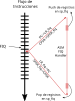
\includegraphics[width=0.95\textwidth]{Vectoring-single-fiq.pdf}\end{center}
 \end{textblock*}
\end{frame}

\begin{frame}[t,fragile]{Ejemplos}
 \begin{textblock*}{\textwidth}(0.4cm,1.5cm) \justifying
   \begin{lstlisting}[basicstyle=\scriptsize,escapechar=\@,numbers=none, frame=single, xleftmargin=20pt, xrightmargin=0pt,]
IRQ-Handler:
    PUSH {r0-r3, r12, lr} /*Almacena registros en la pila */
    BL   identify_source  /*Devuelve direcci@\color{purple}\'o@n del handler en R0*/
    BL   R0               /*Salta al handler (escrito en C o ASM)*/
    POP  {r0-r3, r12, lr} /*Recupera registros de la pila*/
    SUBS pc, lr, #4       /*Retorna utilizando el LR modificado*/
   \end{lstlisting}
 \end{textblock*}
 \begin{textblock*}{\textwidth}(0.4cm,4cm) 
  \begin{itemize}[<+(1)->]\justifying \parskip 0.2cm
   \item La función \textit{\texttt{identify\_source}} es 100\% hardware dependiente, ya que interactúa con el controlador de interrupciones específico incluido en el sistema, para determinar cual de todas las posibles fuentes de interrupción es la responsable del requerimiento.
   \item Regresa en \texttt{\textbf{R0}} la dirección de (puntero a) la función que implementa el handler correspondiente. Elegimos \texttt{\textbf{R0}}, para que \textit{\texttt{identify\_source}} sea compatible con el ABI ARM, y pueda ser invocada también desde un programa escrito en C, si así se lo requiriese.
  \end{itemize}
 \end{textblock*}
\end{frame}

\begin{frame}[t]{Manejo de Interrupciones Anidado}
 \begin{textblock*}{\textwidth}(0.4cm,1.2cm) 
  \begin{itemize}[<+(1)->]\justifying
   \item Anidamiento de interrupciones significa poder aceptar una nueva interrupción antes de finalizar el procesamiento de la interrupción corriente.
   \item Permite alcanzar los requerimientos temporales mediante la priorización de interrupciones urgentes, con mínima demora (latency) en su atención.
   \item El anidamiento por lo general no está impuesto por el hardware.
   \item El costo del anidamiento es, por lo tanto,  mayor complejidad en el software.
   \item Hay un único handler de atención para las diferentes fuentes de interrupción que implementa condiciones adecuadas de priorización.
   \item Debe aceptar re-entrancia, es decir, que estando procesando un handler de interrupción ésta vuelva a repetirse forzando el anidamiento dentro del mismo handler sin perder el estado de máquina.
  \end{itemize}
 \end{textblock*}
\end{frame}
   
\begin{frame}{Manejo de Interrupciones Anidado}
 \begin{textblock*}{\textwidth}(0.4cm,1.2cm) 
  \begin{itemize}[<+->]\justifying   
   \item Un handler de interrupción re-entrante debe salvar el estado IRQ o FIQ antes de conmutar el core al nuevo estado.
   \item Además debe salvar el estado del nuevo modo antes de invocar a la función de anidamiento de interrupciones con las interrupciones habilitadas.
   \item De otro modo, como las interrupciones de hardware pueden ocurrir en cualquier momento (no son determinísticas), puede pisarse el registro de estados original con el de la nueva interrupción y cuando la interrupción original deba retornar al programa interrumpido originalmente, el registro \texttt{\textbf{SPSR}} del modo IRQ o FIQ contiene otro estado, y el programa entra inexorablemente en falla.
   \item Para evitar ésto, el handler anidado debe cambiar a un modo privilegiado en el que deshabilite las interrupciones hasta completar esta tarea.
  \end{itemize}
 \end{textblock*}
\end{frame}

\begin{frame}[fragile]{Manejo de Interrupciones Anidado}
 \begin{textblock*}{\textwidth}(0.4cm,1.2cm)
  \centering 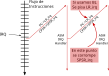
\includegraphics[width=0.55\textwidth]{Vectoring-nested.pdf}
 \end{textblock*}
 \begin{textblock*}{\textwidth}(0.4cm,7.0cm)\justifying
  \only<2-3>{La solución es apilar el \textbf{\texttt{SPSR}} antes de habilitar las interrupciones.}
  \only<4->{Para evitar la corrupción del registro \texttt{\textbf{LR\_irq}}, lo que debe hacerse es switchear a modo Supervisor antes de ejecutar la instrucción de Salto, \textbf{\texttt{BL}}. Se retornará a este estado antes de regresar al handler previo.}
 \end{textblock*}
 \begin{textblock*}{\textwidth}(0cm,7.2cm)
  \begin{onlyenv}<3>
   \begin{lstlisting}[basicstyle=\scriptsize,escapechar=\@,numbers=none, frame=single, xleftmargin=20pt, xrightmargin=0pt,]
SRSFD  sp!,#0x12/*SRS Store Return Status (LR y CPSR).*/
                /*FD: Full Descending, sp: stack, 0x12: modo IRQ.*/
                /*!: luego de la operaci@\color{purple}\'o@n actualiza SP_irq.*/
   \end{lstlisting}
  \end{onlyenv}
 \end{textblock*}
\end{frame}

\begin{frame}{Secuencia de Handler de Interrupciones Anidado}
 \begin{textblock*}{\textwidth}(0.4cm,1.2cm)
  \begin{enumerate}[<+(1)->]\justifying %\parskip 0.3cm
   \item El handler de interrupción debe resguardar todos aquellos registros que puedan ser modificados, incluido \textbf{\texttt{SPSR\_irq}}.
   \item Identificar la fuente de la interrupción y eventualmente limpiar el bit en el hardware externo, para evitar un re disparo eventual de la misma interrupción
   \item Cambiar el core a Modo \texttt{\textbf{System}}, manteniendo el bit \textbf{\texttt{CPSR.I}} seteado (interrupciones deshabilitadas).
   \item Salvar la dirección de retorno en el stack de Modo \texttt{\textbf{System}} (que estará ubicado en la memoria de modo kernel) y habilitar las interrupciones.
   \item Invocar al código del handler específico de la fuente de interrupción.
   \item Al retorno desde éste handler específico, deshabilitar las interrupciones y recuperar la dirección de retorno de excepción desde el stack de Modo \texttt{\textbf{System}}.
   \item Recuperar los registros guardados en el stack de Modo \texttt{\textbf{System}}, incluido el \textbf{\texttt{PC}}, y el \textbf{\texttt{CPSR}}, el cual devolverá el core a su Modo original. Si el bit \textbf{\texttt{SPRS.I}} no estaba seteado, las interrupciones quedarán nuevamente habilitadas.
  \end{enumerate}
 \end{textblock*}
\end{frame}

\begin{frame}[t,fragile]{Ejemplo de Handler de Anidado para IRQ}
 \begin{textblock*}{1.02\textwidth}(0.2cm,1.2cm)
  \begin{lstlisting}[basicstyle=\scriptsize,escapechar=\@,numbers=none, frame=single, xleftmargin=20pt, xrightmargin=0pt,]
IRQ_Handler:
 SUB     lr, lr, #4
 SRSFD   sp!, #0x1f  /*LR_irq y SPSR_irq al stack modo System.*/
 CPS     #0x1f       /*CPS switchea a Modo System.*/
    
 PUSH    {r0-r3, r12}/*Salva contexto en stack Modo System.*/
 AND     r1, sp, #4  /*Si sp est@\color{purple}\'a@ alineado a 8, r1 = 0. Si no, r1 = 4.*/
 SUB     sp, sp, r1  /*Resta 0 o 4 a SP, asegurando stack alineado a 8-byte. */
 PUSH    {r1, lr}    /*Ajuste a 8-byte y LR_sys al stack.*/
    
 BL      id_source   /*Devuelve direcci@\color{purple}\'o@n del handler en R0*/

 CPSIE   i           /*Habilita IRQ con CPS*/
 BL      R0          /*Invoca al handler reentrante*/
 CPSID   i           /*Deshabilita IRQ conCPS*/

 POP     {r1, lr}    /*Recupera LR_sys*/
 ADD     sp, sp, r1  /*Desajusta stack*/
 POP     {r0-r3, r12}/*Recupera los registros*/
 RFE     sp!         /*Retorna desde el stack de Modo System.*/
  \end{lstlisting}
 \end{textblock*}
\end{frame}

\section{GIC Architecture}
\subsection{Generic Interrupt Controler}
\begin{frame}[t]{Parte de una Arquitectura}
 \begin{textblock*}{\textwidth}(0.4cm,1.2cm)
  \begin{block}{Generic Interrupt Controller}
   \begin{itemize}[<+(1)->]\justifying
    \item Comprende un set de recursos de hardware para manejar interrupciones en sistema con un solo core o múltiples cores. 
    \item Define un conjunto de registros mapeados en memoria, que permiten gestionar las diferentes fuentes de interrupción y controlar su comportamiento, y en el caso de sistemas multicore, enrutar interrupciones a un core individual determinado.
    \item Permite habilitar y deshabilitar individualmente las diferentes fuentes de interrupción de hardware, priorizarlas por hardware, y generar interrupciones de software. 
    \item Provee soporte para las Extensiones de Seguridad.
    \item Acepta interrupciones a nivel del SoC y las mapea en un core individual como IRQ o FIQ.
   \end{itemize}
  \end{block}
 \end{textblock*}
\end{frame}

\begin{frame}[t]{Dos bloques funcionales (perspectiva del software)}
 \begin{textblock*}{\textwidth}(0.4cm,1.1cm)
  \begin{block}{Distribuidor}
   \begin{itemize}[<+(1)->]\justifying
    \item Tiene cableadas todas las fuentes de interrupción del sistema. 
    \item Se compone de un conjunto de registros que controlan las propiedades de cada fuente de interrupción de manera individual, tales como prioridad, estado, seguridad, información de vectorización, y habilitación.
    \item Determina cual de las interrupciones será enviada a un core a través de la \textbf{\textit{Interfaz con la CPU}}.  
   \end{itemize}
  \end{block}
 \end{textblock*}
 \only<5->{
 \begin{textblock*}{\textwidth}(0.4cm,5.2cm)
  \begin{block}{Interfaz con la CPU}
  \begin{itemize}[<+(1)->]\justifying
   \item Es la entrada por donde el core recibe una interrupción. 
   \item Contiene una serie de registros para enmascarar, identificar y controlar el estado de las interrupciones enviadas al core. 
   \item Hay una \textbf{\textit{interfaz con la CPU}} por cada core del sistema.
  \end{itemize}
  \end{block}
 \end{textblock*}
 }
\end{frame}

\begin{frame}[t]{Identificación de interrupciones}
 \begin{textblock*}{\textwidth}(0.4cm,1.2cm)
  \begin{block}{\textbf{\textit{Interrupt ID}}}\justifying
   \only<2->{Las fuentes de interrupciones se identifican unívocamente en el software mediante un número denominado \textbf{\textit{Interrupt ID}}.}
   
   \only<3->{En base a este número el software puede invocar al handler de interrupción correspondiente.}
   
   \only<4->{Los valores específicos de \textbf{\textit{Interrupt ID}}, se determinan en el diseño del sistema.}
  \end{block}
  \only<5->{Hay tres tipos de Interrupciones:}\parskip 0.3cm
  \begin{itemize}[<+(5)->]\parskip 0.3cm
   \item Software Generated Interrupts (SGI)
   \item Private Peripheral Interrupts (PPI)
   \item Shared Peripheral Interrupts (SPI)
  \end{itemize}
 \end{textblock*}
\end{frame}

\begin{frame}[t]{Software Generated Interrupts}
 \begin{textblock*}{\textwidth}(0.4cm,1.5cm)
  \begin{itemize}[<+(1)->]\justifying \parskip 0.2cm
   \item Se generan escribiendo desde el software en el registro \texttt{\textbf{ICDSGIR}}, \textit{Software Generated Interrupt Register,} específico del \textbf{\textit{Distribuidor}}.
   \item Su principal aplicación es la comunicación inter core.
   \item Pueden destinarse a todos los cores o a un grupo seleccionable de cores. 
   \item Para esto último se reservan los números de interrupción 0 a 15.
   \item El número exacto que se utiliza para este fin, queda a criterio del diseñador del software de manejo de interrupciones.
  \end{itemize}
 \end{textblock*}
\end{frame}

\begin{frame}[t]{Private Peripheral Interrupts}
 \begin{textblock*}{\textwidth}(0.4cm,1.5cm)
  \begin{itemize}[<+(1)->]\justifying \parskip 0.2cm
   \item Se trata de una interrupción generada por una fuente de interrupción privada o exclusiva de un core determinado.
   \item Se reservan para este tipo los números 16 a 31.
   \item El número asignado es identificatorio de una fuente privada del core. 
   \item Puede coincidir con la misma fuente de otro core.
   \item Un claro ejemplo es el temporizador de cada core
  \end{itemize}
 \end{textblock*}
\end{frame}

\begin{frame}[t]{Shared Peripheral Interrupts}
 \begin{textblock*}{\textwidth}(0.4cm,1.5cm)
  \begin{itemize}[<+(1)->]\justifying \parskip 0.2cm
   \item Se trata de una interrupción generada por una fuente de interrupción que puede ser enrutada a mas de un core.
   \item Se reservan para este tipo los números 32 a 1020.
   \item Un dispositivo SPI es el caso mas claro, entre otros.
   \item Su interrupción puede ser derivada a cualquiera de los cores del sistema.
  \end{itemize}
 \end{textblock*}
\end{frame}


\begin{frame}[t]{Señalización de una interrupción}
 \begin{textblock*}{\textwidth}(0.4cm,1.5cm)
  \begin{itemize}[<+(1)->]\justifying \parskip 0.4cm
   \item \textbf{\color{Blue1}Edge-Triggered}: Disparo por flanco. Requiere que la señal en la entrada de la fuente de interrupción pase del estado bajo al estado alto (Flanco ascendente de disparo). Permanece vigente hasta que se limpie.
   \item \textbf{\color{Blue3}Level-Triggered}: Disparo por nivel. Se considera que una fuente de interrupción está activa si el nivel de tensión aplicado en su estado es alto.
  \end{itemize}
 \end{textblock*}
\end{frame}

\begin{frame}[t]{Estados de una interrupción}
 \begin{textblock*}{\textwidth}(0.4cm,1.5cm)
  \begin{itemize}[<+(1)->]\justifying \parskip 0.4cm
   \item \textbf{\color{Blue1}Inactive}: Significa que la interrupción aun no ha sido enviada.
   \item \textbf{\color{Blue2}Pending}: Significa que la interrupción ha sido enviada pero está esperando ser atendida por el core. Cuando están en este estado son candidatas a ser enviadas a la \textit{\textbf{Interfaz con la CPU}}, y mas tarde nuevamente al core.
   \item \textbf{\color{Blue3}Active}: Indica que la interrupción ha sido atendida por el core y está siendo procesada
   \item \textbf{\color{Blue4}Active and Pending}: Indica que el core está procesando esta fuente de interrupción pero el GIC tiene un nuevo requerimiento pendiente para esa misma fuente.
  \end{itemize}   
 \end{textblock*}
\end{frame}


\begin{frame}[t]{Procesamiento de una interrupción en el GIC}
 \begin{textblock*}{\textwidth}(0.4cm,1.5cm)
  \begin{enumerate}[<+(1)->]\justifying \parskip 0.3cm \seti
   \item La prioridad de las diferentes fuentes de interrupción y la lista de cores a los que cada una puede ser derivada se maneja en el \textbf{\textit{Distribuidor}}.
   \item Cuando se recibe una interrupción de una fuente determinada, ésta se establece en el \textbf{\textit{Distribuidor}} en estado \textbf{\textit{\color{Blue3}Pending}} (o \textbf{\textit{\color{Blue4}Active and Pending}} en el caso en que esa fuente de interrupción haya generado un requerimiento previo que sigue estando en proceso)
   \item El \textbf{\textit{Distribuidor}}, determina entre las pendientes aquella de mayor prioridad y la deriva a la \textit{\textbf{Interfaz con la CPU}} del core correspondiente.
   \item La \textit{\textbf{Interfaz con la CPU}} envía una señal de interrupción por la entrada \texttt{\textbf{FIQ}} o la entrada \texttt{\textbf{IRQ}} de la CPU.
   \seti
  \end{enumerate}
 \end{textblock*}
\end{frame}

\begin{frame}[t]{Procesamiento de una interrupción en el GIC}
 \begin{textblock*}{\textwidth}(0.4cm,1.2cm)
  \begin{enumerate}[<+->]\justifying \parskip 0.15cm \conti
   \item El core ejecuta el handler de la excepción \textbf{\texttt{IRQ}} o \textbf{\texttt{FIQ}}, de acuerdo con la entrada por la que ha ingresado el requerimiento de interrupción.
   \item El software lee el \textbf{\textit{Interrupt ID}} de los registros del GIC .
   \item Con éste número, invoca al handler específico de interrupción del periférico correspondiente a la fuente de interrupción recibida, para finalmente atender el requerimiento concreto.
   \item Una vez finalizado éste handler, el software debe acceder al registro de la \textit{\textbf{Interfaz con la CPU}},  para señalar el fin de la atención de la interrupción.
   \item El GIC actualiza el estado de la interrupción en sus registros. Oscilará entre \textbf{\color{Blue2}Active} y \textbf{\color{Blue3}Pending}, mientras la interrupción esté siendo atendida, y quedará en \textbf{\color{Blue1}Inactive} una vez atendida.
  \end{enumerate}
 \end{textblock*}
\end{frame}

\begin{frame}[t]{Configuración}
 \begin{textblock*}{\textwidth}(0.4cm,1.5cm)
  \begin{itemize}[<+(1)->]\justifying \parskip 0.2cm
   \item El GIC se presenta al software como un conjunto de registros memory-mapped. Se accede como si fuera un periférico.
   \item El bloque \textbf{\textit{Distribuidor}} es común a todos los cores, pero la \textit{\textbf{Interfaz con la CPU}} banquea sus registros de manera individual para cada core. 
   \item Cada core utiliza el mismo rango de direcciones para acceder a su propia \textbf{\textit{Interfaz con la CPU}}.
   \item Ningún core tiene acceso a los registros de la \textbf{\textit{Interfaz con la CPU}} de otro core. \textbf{Nunca}.
   \item El espacio de registros memory-mapped correspondiente a los registros del \textbf{\textit{Distribuidor}} permite a  todos los cores configurar diferentes propiedades.
  \end{itemize}
 \end{textblock*}
\end{frame}

\begin{frame}[t]{Configuración - Propiedades}
 \begin{textblock*}{\textwidth}(0.4cm,1.2cm)
  \begin{itemize}[<+(1)->]\justifying% \parskip 0.2cm
   \item Prioridad. Permite al \textbf{\textit{Distribuidor}} determinar cual será la siguiente fuente de interrupción a derivar hacia la \textbf{\textit{Interfaz con la CPU}}.
   \item Es posible configurar para cada core un nivel mínimo de prioridad para que una fuente le sea derivada.
   \item Configuración de la Interrupción. Determina si la línea de hardware se activa por flanco o por nivel.
   \item Target de la interrupción. Lista de cores hacia los que se puede derivar el requerimiento de interrupción.
   \item Habilitación/Deshabilitación. Solo las interrupciones de fuentes habilitadas serán derivadas por el \textbf{\textit{Distribuidor}} a un core cuando pasan a estado \textbf{\textit{\color{Blue2}Pending}}. 
   \item La seguridad de la interrupción. Esto es, si el handler va a ejecutar en modo Seguro o Normal.
   \item El estado.
  \end{itemize}
 \end{textblock*}
\end{frame}

\begin{frame}[t]{Inicialización}
 \begin{textblock*}{\textwidth}(0.4cm,1.2cm)
  \begin{itemize}[<+(1)->]\justifying% \parskip 0.2cm
   \item El GIC está deshabilitado luego del reset. Debe ser inicializado antes de comenzar a aceptar requerimientos de interrupción.
   \item El \textbf{\textit{Distribuidor}} y la \textbf{\textit{Interfaz con la CPU}} se habilitan por separado.
   \item Se inicializan todas las características recién descriptas para el \textbf{\textit{Distribuidor}} y se lo habilita a través de su Registro de control.
   \item Para cada \textbf{\textit{Interfaz con la CPU}} se programan la máscara de prioridades y los ajustes de preemption.
   \item Cada \textbf{\textit{Interfaz con la CPU}} debe ser habilitada por su core. 
   \item Esto deja al GIC listo para enviar requerimientos de interrupción.
   \item Antes de aceptar interrupciones el core debe inicializar el vector de interrupciones apuntando a los handlers previstos para cada interrupción ARM.
   \item Finalmente en el \textbf{\texttt{CPSR}} de cada core, se debe habilitar las interrupciones.
  \end{itemize}
 \end{textblock*}
\end{frame}

\begin{frame}[t]{Inicialización}
 \begin{textblock*}{\textwidth}(0.4cm,1.2cm)
  \begin{block}{Opciones de Habilitación/Deshabilitación}\justifying
   \only<2->{Deshabilitar el \textbf{\textit{Distribuidor}}, deshabilita el sistema de interrupciones completo para la totalidad de los cores.}
   
   \only<3->{Deshabilitar el bloque de \textbf{\textit{Interfaz con la CPU}} equivale a deshabilitar las interrupciones de un core individual seteando el bit \texttt{\textbf{CPSR.I}}.}
   
   \only<4->{También pueden habilitarse o deshabilitarse, en forma individual las interrupciones en el \textbf{\textit{Distribuidor}}.}
  \end{block}
 \end{textblock*}
\end{frame}

\begin{frame}[t]{Procesamiento de una interrupción en el Software}
 \begin{textblock*}{\textwidth}(0.4cm,1.2cm)
  \begin{enumerate}[<+(1)->]\justifying \parskip 0.125cm 
  \seti
   \item El core que recibe la interrupción vectoriza al handler de alto nivel (salta a la dirección de la tabla de vectores de Interrupción).
   \item Lee el \textit{Interrupt Acknowledge Register} de la \textbf{\textit{Interfaz con la CPU}}, y obtiene de allí el \textbf{\textit{Interrupt ID}}.
   \item Al detectar esta lectura el \textbf{\textit{Distribuidor}} setea la fuente de interrupción en estado \textbf{\textit{\color{Blue2}Active}}.
   \item Con el \textit{\textbf{Interrupt ID}} el handler de alto nivel determina cual es el handler específico de la interrupción, y lo puede invocar.
   \item Cuando el handler específico termina su ejecución retorna al handler de alto nivel que escribe en el \textbf{\textit{End Of Interrupt Register}} de la \textbf{\textit{Interfaz con la CPU}}.
   \item Si el estado estaba \textbf{\textit{\color{Blue2}Active}}, lo cambia a \textbf{\textit{\color{Blue1}Inactive}}, y si estaba \textbf{\textit{\color{Blue4}Active and Pending}} lo cambia a \textbf{\textit{\color{Blue3}Pending}}
   \seti
  \end{enumerate}
 \end{textblock*}
\end{frame}

\end{document}
